\documentclass{../notatki}

\title{Elektryczność i Magnetyzm}

\usetikzlibrary{calc}

\begin{document}

\tableofcontents

\section{Literatura}

\begin{itemize}
  \item E. M. Purcell, D. J. Morin "Electricity and Magnetism"
  \item R. Shankar "Fundamentals of Physics II"
  \item OpenStax
    \href{https://assets.openstax.org/oscms-prodcms/media/documents/College_Physics_2e-WEB_7Zesafu.pdf#%5B%7B%22num%22%3A2876%2C%22gen%22%3A0%7D%2C%7B%22name%22%3A%22XYZ%22%7D%2C0%2C734%2C0%5D}{"College
    Physics"}
\end{itemize}

\section{Cząstki}

Elektryczność jest zjawiskiem, wynikającym z oddziaływań pomiędzy nukleonami.
Wyróżniamy trzy nukleony: proton, neutron i elektron. Proton ma ładunek dodatni,
neutron jest obojętny, a elektron ma ładunek ujemny. Proton i neutron znajdują
się w jądrze atomowym, które choć zmienne w wyniku reakcji jądrowych, jest
stabilne w warunkach normalnych. Elektrony z kolei krążą wokół jądra w tzw.
chmurze elektronowej. W wyniku oddziaływań pomiędzy innymi nukleonami elektrony
mogą być oderwane od atomu, tworząc jon dodatni lub ujemny. Tymczasowy brak
równowagi, gradient ładunku, w materiale złożonym z kilku cząstek
jest przyczyną zjawisk elektrycznych.

\subsection{Przewodniki}

Wyróżniamy grupę materiałów, które w wyniku ich struktury atomowej pozwalają na
swobodny transfer elektronów i powstawanie gradientu ładunku. Są to przewodniki.
Metale w wyniku istnienia specjalnych wiązań chemicznych są dobrymi
przewodnikami.
Podobnie roztwory elektrolityczne, w których jony mogą swobodnie
przemieszczać się
w roztworze. W przeciwieństwie do przewodników, izolatory nie
pozwalają na swobodny
transfer elektronów. W wyniku tego nie powstaje gradient ładunku.

\subsection{Ładunek}

Ładunek danej dyskretnej cząsteczki jest wielkością skalarną określoną wzorem:
$$
q = n \cdot e
$$
gdzie $e$ to ładunek elementarny($1.6 \cdot 10^{-19} C$), a $n$ to liczba
cząsteczek.
\textbf{Suma ładunków w układzie izolowanym jest stała.}

\subsection{Elektryzowanie}

W wyniku różnych oddziaływań pomiędzy ciałami, mogą one nabrać
ładunku. Wyróżniamy
kilka metod elektryzowania ciał. W każdej z nich powstaje gradient ładunku.

\subsubsection{Elektryzowanie przez tarcie}

W wyniku tarcia między ciałami, elektrony mogą być przenoszone z
jednego ciała na
drugie. W wyniku tego jedno ciało nabiera ładunku dodatniego, a drugie ujemnego.

\subsubsection{Elektryzowanie przez dotyk}

W momencie, w którym dotkniemy dwa ciała o różnym ładunku
przewodnikiem, elektrony
przenoszą się z ciała o większym ładunku do ciała o mniejszym
ładunku. W wyniku tego
oba ciała nabierają ładunku o wartości pośredniej.

\subsubsection{Elektryzowanie przez indukcję}

W wyniku zbliżenia ciała o ładunku do ciała obojętnego, ładunek
w ciele obojętnym jest przemieszczany w wyniku oddziaływań pomiędzy
ładunkami. W wyniku tego ciało obojętne nabiera ładunku. W materiałach
przewodzących ładunek jest przemieszczany swobodnie, w izolatorach gradient
powstaje w wyniku polaryzacji cząsteczek.

\section{Prawo Coloumba}

Ciała naelektryzowane oddziałują na siebie zgodnie z prawem Coloumba:
$$
\vec{F_E} = k \cdot \frac{q_1 \cdot q_2}{r^2} \cdot \vec{r}
$$
gdzie $k$ to stała elektrostatyczna($\frac{1}{4\pi\epsilon_0}$,
$\epsilon_0\approx8.854\cdot10^{-12}\frac{E}{m}$).

\subsection{Zasada superpozycji}

Siła wypadkowa działająca na ciało naelektryzowane jest sumą sił
działających na to ciało ze strony innych ciał.
$$
\vec{F_w} = k \cdot \sum_{j=1}^{n} \frac{q_1 \cdot q_j}{r^2} \cdot \vec{r}
$$

\subsection{Przykład}

\begin{figure}[h]
  \centering
  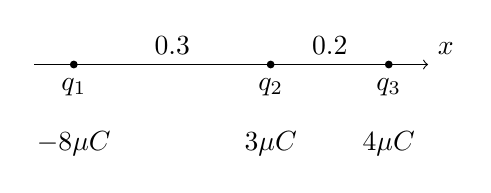
\begin{tikzpicture}
    \draw[->] (0,0) -- (5,0) node[above right] {$x$};
    \node[circle,fill,inner sep=1pt,label=below:$q_1$] (q1) at (0.5,0) {};
    \node[circle,fill,inner sep=1pt,label=below:$q_2$] (q2) at (3,0) {};
    \node[circle,fill,inner sep=1pt,label=below:$q_3$] (q3) at (4.5,0) {};
    \draw[] (q1) -- (q2) node[midway,above] {$0.3$};
    \draw[] (q2) -- (q3) node[midway,above] {$0.2$};
    \node[below of=q1] {$-8\mu C$};
    \node[below of=q2] {$3\mu C$};
    \node[below of=q3] {$4\mu C$};
  \end{tikzpicture}
\end{figure}
$$
\vec{F_{31}} = k \cdot \frac{q_1 \cdot q_3}{r^2} = k \cdot \frac{-8\cdot
4}{0.5^2} = -1.2 N
$$
$$
\vec{F_{32}} = k \cdot \frac{q_1 \cdot q_2}{r^2} = k \cdot \frac{3\cdot
4}{0.2^2} = 2.7 N
$$

\section{Pole elektryczne}

Pole elektryczne jest polem wektorowym, które opisuje siłę działającą na
naelektryzowane ciało. Siła pola elektrycznego zależy od ładunku,
tworzącego pole elektryczne, oraz od odległości od ładunku.

\subsection{Linia pola elektrycznego}

Do obrazowego przedstawienia pola elektrycznego używamy linii pola
elektrycznego. Linie pola elektrycznego to linie które w każdym punkcie są
styczne do wektora siły pola elektrycznego. Są one przedstawiane jako dyskretne
linie, lecz w rzeczywistości pole elektryczne jest ciągłe.

\subsection{Natężenie pola elektrycznego}

Natężenie pola elektrycznego to wielkość wektorowa, która opisuje siłę
działającą na jednostkowy ładunek w danym punkcie pola elektrycznego.
$$
\vec{E}(r) = k \cdot \frac{|q|}{r^2} \cdot \vec{r}
$$
Gdzie $r$ to odległość od ładunku, a $q$ to ładunek, tworzący pole
elektryczne.
$$
\vec{F_E} = q \cdot \vec{E}(r)
$$

\begin{figure*}[h]
  \centering
  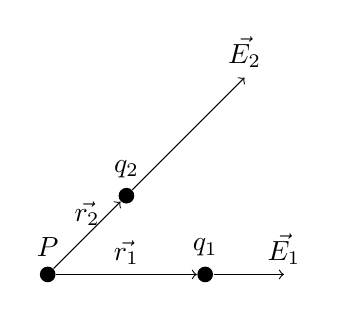
\begin{tikzpicture}
    \node[circle, fill, inner sep=2pt, label=above:$P$] (p) at (0,0) {};
    \node[circle, fill, inner sep=2pt, label=above:$q_1$] (q1) at (2,0) {};
    \draw[->] (p) -- (q1) node[midway, above] {$\vec{r_1}$};
    \draw[->] (q1) -- (3,0) node[above] {$\vec{E_1}$};
    \node[circle, fill, inner sep=2pt, label=above:$q_2$] (q2) at (1,1) {};
    \draw[->] (q2) -- (2.5,2.5) node[above] {$\vec{E_2}$};
    \draw[->] (p) -- (q2) node[midway, above] {$\vec{r_2}$};
  \end{tikzpicture}
  \caption{Ilustracja natężenia pola elektrycznego, $|\vec{r_1}| <
  |\vec{r_2}| \rightarrow |\vec{E_1}| > |\vec{E_2}|$}
\end{figure*}

\subsection{Pole elektryczne przewodnika}

Zewnętrzne pole elektryczne powoduje, że ładunki się przemieszczają wewnątrz
przewodnika. Powstaje w ten sposób pole elektryczne wewnętrzne
przewodnika, które
jest przeciwnie skierowane do pola zewnętrznego. W wyniku tego pole elektryczne
wewnątrz przewodnika jest równe 0.

\begin{figure}[h]
  \centering
  \begin{tikzpicture}
    \begin{scope}
      \clip (-1.5,1) rectangle (1.5,1.5);
      \draw (0,0) circle(1.5);
    \end{scope}
    \draw[->] (0,1.5) -- (0,2.5) node[above] {$\vec{E_n}$};
    \draw[->] (0,1.5) -- (1,1.5) node[above] {$\vec{E_t}$};
    \node at (3, 3) {$\vec{E_n} \ne 0, \vec{E_t} = 0$};
  \end{tikzpicture}
  \caption{Pole elektryczne na powierzchni przewodnika}
\end{figure}

\section{Dipol elektryczny}

Dipol elektryczny to układ dwóch ładunków o równych wartościach, lecz
przeciwnych znakach. W wyniku tego układu powstaje pole elektryczne, które
jest zależne od odległości między ładunkami. W wyniku tego dipol elektryczny
jest zawsze zorientowany w kierunku od ładunku dodatniego do ujemnego.
\begin{figure}[h]
  \centering
  \begin{tikzpicture}
    \node[circle,fill,inner sep=1pt,label=below:$q_+$] (q1) at (0,0) {};
    \node[circle,fill,inner sep=1pt,label=below:$q_-$] (q2) at (2,0) {};
    \draw[-] (q1) -- (q2) node[midway,above] {$d$};
  \end{tikzpicture}
\end{figure}

Poszczególne bieguny dipola elektrycznego oddziałują na inne ciała osobno.
Przez to, np.: ciała pozytywnie naładowane będą doświadczały różnej siły
działającej ze strony dipola, w zależności od pozycji ciała względem dipola.
Energia dipola elektrycznego to:
$$
E = E_+ + E_-
$$
Co za tym idzie, dla $d \rightarrow 0$ dipol zaczyna zachowywać się jak
punktowy ładunek.

Dla dipola mamy moment dipolowy $p = qd$. Gdy dipol o moment dipolowym $p$ jest
umieszczony w jednorodnym polu elektrycznym $\vec{E}$, to na dipol działa moment
siły $\vec{\tau} = \vec{p} \times \vec{E}$.

\section{Ciągłe rozkłady ładunków}

Nie zawsze ciała mają dyskretne ładunki. W takich przypadkach rozważamy rozkłady
powierzchniowe, liniowe i objętościowe ładunków, w zależności co dzielimy
na infinitesimalne elementy.

\subsection{Gęstość liniowa ładunku}

$$
\lambda = \lim_{\Delta s \rightarrow 0} \frac{\Delta q}{\Delta s} =
\frac{dq}{ds}
$$
$$
q = \int \lambda ds
$$

\subsection{Gęstość powierzchniowa ładunku}

$$
\sigma = \lim_{\Delta A \rightarrow 0} \frac{\Delta q}{\Delta A} =
\frac{dq}{dA}
$$
$$
q = \int \sigma dA
$$

\subsection{Gęstość objętościowa ładunku}

$$
\rho = \lim_{\Delta V \rightarrow 0} \frac{\Delta q}{\Delta V} =
\frac{dq}{dV}
$$
$$
q = \int \rho dV
$$

\subsection{Natężenie pola elektrycznego}

$$
\vec{E} = k \cdot \int \frac{dq}{r^2} \cdot \vec{r}
$$
$$
dq =
\begin{cases}
  \lambda ds & \text{dla ładunku liniowego} \\
  \sigma dA & \text{dla ładunku powierzchniowego} \\
  \rho dV & \text{dla ładunku objętościowego}
\end{cases}
$$

\section{Prawo Gaussa}

$$
\Phi_E = \oint \vec{E} \cdot d\vec{s} = \frac{q}{\epsilon_0}
$$
gdzie $\vec{s}$ to wektor powierzchni, a $\vec{E}$ to pole elektryczne, które
przechodzi przez tę powierzchnię.

\begin{figure*}[h]
  \centering
  \resizebox{0.8\textwidth}{!}{
    \begin{minipage}{0.5\textwidth}
      \begin{tikzpicture}
        \node (start) at (0,0) {$-\infty$};
        \node (end) at (0,4) {$\infty$};
        \draw[-] (start) -- (end) node[midway,left] {$\lambda$};
        \node[circle,fill,inner sep=2pt] (s) at (2,2) {};
        \draw[->] (s) -- (3, 2) node[above] {$\vec{s}$};
        \draw[dotted] (0, 2) -- (s) node[midway, above] {$r$};
      \end{tikzpicture}
    \end{minipage}
    \begin{minipage}{0.5\textwidth}
      Linia jest nieskończona, jako uproszczenie. Jeśli linia byłaby skończona,
      to trzeba by brać pod uwagę zmienne pole elektryczne na końcach linii.
      \\\\
      Aby ułatwić obliczenia tworzymy przestrzeń zamkniętą, która zawiera linię.
      Ta przestrzeń otacza linię, tak aby $\vec{E} \| d\vec{s}$. Następnie
      obliczamy pole elektryczne w każdym punkcie przestrzeni zamkniętej.
      $$
      \frac{q}{\epsilon_0} = E \cdot 2 \pi rl
      $$
      $$
      E = \frac{\lambda}{2\pi\epsilon_0 r}
      $$
    \end{minipage}
  }
  \caption{Prawo Gaussa dla ładunku liniowego w nieskończonej linii}
\end{figure*}

\section{Potencjał elektryczny}

Potencjał elektryczny to wielkość skalarna, która opisuje pracę wykonaną nad
jednostkowym ładunkiem, aby przenieść go z nieskończoności do danego punktu.

\subsection{Własności sił zachowawczych}

Siły zdefiniowane przez potencjał są siłami zachowawczymi.
$$
\vec{F} = - \nabla U = - (\frac{\partial U}{\partial x}, \dots)
$$
Oznacza to, że praca wykonana nad ładunkiem w zamkniętym obwodzie jest równa 0.
Również to oznacza, że $U_1 - U_2 = - \oint F$

\subsection{Potencjał pola elektrycznego}

$$
V = V_1 - V_2 = - \int_{r_1}^{r_2} E(r) \cdot dr
$$
$$
E = - \nabla V
$$
Zatem pole elektryczne jest gradientem potencjału elektrycznego. I na odwrót,
potencjał elektryczny jest całką pola elektrycznego.
$$
V(r) = \frac{q}{4\pi\epsilon_0 r}
$$
Co za tym idzie siła pola elektrycznego jest gradientem potencjału
energii elektrycznego.
$$
U = q \cdot V
$$
$$
F_E = q \cdot E = - \nabla U
$$

\section{Kondensatory}

Kondensatory to układy elektryczne, które przechowują elektryczną energię
potencjalną. Składają się z dwóch przewodników, oddzielonych dielektrykiem.
Dla kondensatora mamy pojemność $C = \frac{Q}{V}$, gdzie $Q$ to ładunek, a $V$
to napięcie między przewodnikami.
\begin{figure*}[h]
  \centering
  \resizebox{0.8\textwidth}{!}{
    \begin{minipage}{0.5\textwidth}
      \centering
      \begin{tikzpicture}
        \draw (0,0) to[battery] (0,4);
        \draw (0,4) -- (2,4) to[C, l=$C_1$] (2,0) -- (0,0);
        \draw (2,4) -- (4,4) to[C, l=$C_2$] (4,0) -- (2,0);
      \end{tikzpicture}
      \caption{Kondensatory połączone równolegle.}
    \end{minipage}
    \begin{minipage}{0.5\textwidth}
      \centering
      \begin{tikzpicture}
        \draw (0,0) to[battery] (0,4);
        \draw (0,4) -- (2,4) to[C, l=$C_1$] (2,2) to[C, l=$C_2$] (2,0) -- (0,0);
      \end{tikzpicture}
      \caption{Kondensatory połączone szeregowo.}
    \end{minipage}
  }
\end{figure*}
Kondensatory połączone równolegle mają sumaryczną pojemność $C_{tot}
= C_1 + C_2$. Z kolei kondensatory połączone szeregowo mają sumaryczną pojemność
$C_{tot} = \frac{1}{\frac{1}{C_1} + \frac{1}{C_2}}$.

\end{document}
